% !TeX program = xelatex
\documentclass{ctexart}
\usepackage{template_by_mny}

\title{傅里叶光学实验报告}
\class{物理 32}
\name{冯家琦/周方远}
\id{2023011338}

\begin{document}
\maketitle

\begin{abstract}
  我们在基物课上学习了光的衍射现象与光栅的原理,这次实验我们使用分光计,运用衍射光栅测
  光的波长,从而可以更加深刻理解我们课上学的光栅衍射公式。
\end{abstract}

\section{实验原理}
  \subsection{测定光栅常数和光波波长}
    理想的光栅可看作是许多平行的、等距离的和等宽的狭缝。

    设有一光栅常数 d=AB 的光栅 G。有一束平行光与光栅法线成
    角度 i,入射于光栅上产生衍射,如图 所示。

    若衍射相干加强从而产生明亮的条纹,则光程差满足方程
    \begin{equation}\label{eq:diffraction}
      d (\sin{\varphi} \pm \sin{i}) = m\lambda 
    \end{equation}
    入射光线和衍射光线都在光栅法线的同侧时取正号;两者分居法线异侧时取负号。式中的 m 为衍
    射光谱的级次,m 为 0,$\pm1$,$\pm2$ 等,m 的符号取决于光程差的符号。

    在光线正入射的情形下,i=0,则式\eqref{eq:diffraction}变成
    \begin{equation}
      d \sin{\varphi_m} = m\lambda
    \end{equation}
    从而可用分光计测出衍射角$\varphi_m$,从已知波长可以测出光栅常数$d$。
    \begin{figure}[htbp]
      \centering
      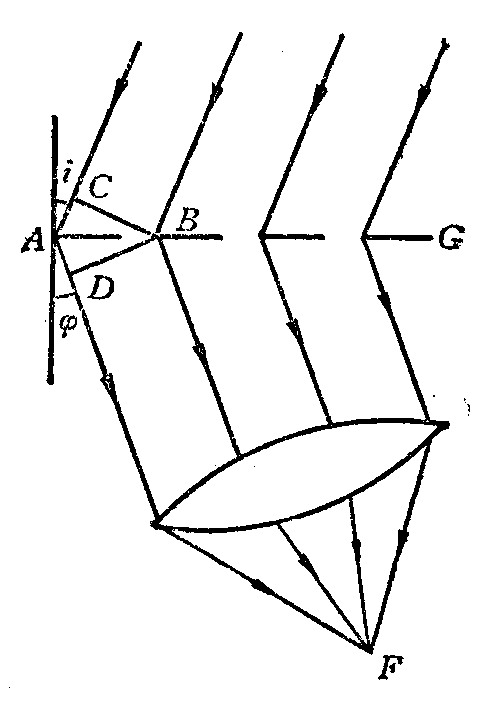
\includegraphics[width=0.2\textwidth,height=0.25\textwidth]{图片.png}
      \caption{光栅衍射}
      \end{figure} 
  \subsection{用最小偏向角法测定光波波长}
  若与入射线同在光栅法线一侧,类似的有
  \begin{equation}\label{eq:diffraction2}
    d (\sin{\varphi} + \sin{i}) = m\lambda 
  \end{equation}
  如图所示
  \begin{figure}[htbp]
    \centering
    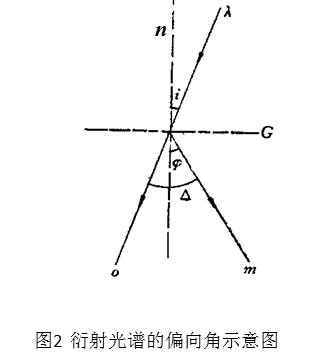
\includegraphics[width=0.2\textwidth,height=0.25\textwidth]{图片2.png}
    \end{figure} 
  偏向角$\Delta =\varphi + i$,当$\varphi=i$时$\Delta$最小,记为$\delta $称为最小偏向角,此时有
  \begin{equation}\label{eq:diffraction2}
    2d \sin{\delta / 2} = m\lambda \qquad  m=0,1,2…
  \end{equation}
\section{实验仪器及实验步骤}
  仪器:分光计,光栅,汞灯
  \subsection{调节望远镜}
    \subsubsection{调节望远镜适合于观察平行光}
      先粗调目镜与叉丝的距离。然后将平面镜放在小平台上,点亮望远镜上的小灯,,缓慢转动小平台,从望远镜中寻
      找镜面反射回来的绿+字像或绿光斑。找到+字像或绿光斑后,轻轻旋转“望远镜调焦旋钮”,从目镜中
      看到清晰的+字像
    \subsubsection{调节望远镜光轴垂直于分光计主轴}
    先从望远镜中看到由平面镜的一面反射的+字像,采取逐步减半逼近法:先调小平台下的螺钉使+字像与叉丝上交点之间的上下距离减
    半,再调节望远镜的俯仰角调节螺钉使像与叉丝上交点重合,然后转动平台 180°进行
    同样调节,反复几次便可很快调好。
    \subsection{调节平行光管}
    调节狭缝和透镜间的距离,从望远镜中看到的是一清晰的狭缝像,到狭缝像的中点与叉丝中心交点重合
    \subsection{在光线垂直入射的情形下,即$i=0$时,测定光栅常数和光波波长}
    调节使光栅平面与平行光管的光轴垂直,光栅刻线(缝)与分光计主轴平行,
    然后测量零级左右两侧各对应级次的衍射线的夹角$2\varphi _m$
    \subsection{在$i=15^{\circ}$时,测定汞灯光谱中波长较长(579.1nm)
    的黄线的波长。}
    使光栅平面法线与平行光管光轴的夹角(即入射角)等于$15^{\circ}$,同时记下入射光方
位和光栅平面的法线方位。然后测定波长较长的黄线的衍射角
    \subsection{用最小偏向角法测定波长较长(579.1nm)的黄线的波长}
      改变入射角,当目镜中谱线折返时,即为最小偏向角的位置,从而可由该谱线
      的方位及零级谱线的方位(即入射光的方位)测出最小偏向角$\delta$。

\section{实验内容}


\section{总结}
\begin{itemize}
  \item 对光波衍射现象和光栅有了更深的了解
  \item 学会了分光计的操作方法
\end{itemize}
\end{document}